\section{Linear gap in complexity length}
\label{sec:line-gap-compl}

\subsection{An example of counting in product regions}
\label{sec:an-example-counting}

Before we define complexity length, we will look at an example that illustrates why we need complexity length.
Theorem 1.3 of \textcite{10.1215/00127094-1548443} proves an estimate on the volume of balls in Teichmüller space.
From this volume estimate, we can obtain an estimate on the cardinality of net points of an $(\vepn, 2 \vepn)$-net $\net$.
\begin{theorem}[Theorem 1.3 of \cite{10.1215/00127094-1548443}]
  \label{thm:abem}
  For a point $p$ in $\teich(S)$ (where $S$ is a genus $g$ surface with $b$ boundary components), the number of net points in a ball of radius $R$ centered at the origin satisfies the following asymptotic as $R$ goes to $\infty$.
  \begin{align*}
    \#\left( \net \cap B_R(p) \right) \emul \exp((6g-6 + 2b)R)
  \end{align*}
  Here, the multiplicative and additive constants showing up in $\emul$ only depend on $p$ and $\vepn$.
\end{theorem}

Suppose now that we want to use the above theorem to count net points in a product region.
More concretely, let $p$ be a point in $\teich(S)$ such that a non-separating curve $\gamma$ is very short: $\ell_{\gamma}(p) \leq \delta \cdot \exp(-R_0)$, for some $\delta > 0$, and some large $R_0$, and we want to estimate the cardinality of $\net \cap B_R(p)$ for $R < R_0$.
Note that since $R < R_0$, the ball $B_R(p)$ is still contained in the product region of Teichmüller space where $\ell_\gamma \leq \delta$.

Since the entire ball $B_R(p)$ is in a product region, we have by Minsky's product region theorem (see Theorem \ref{thm:prno} for a precise statement) that the ball decomposes (up to an additive error) as the
product of a ball in $\teich(S \setminus \gamma)$ and ball in $\mathbb{H}$ (which corresponds to the length and twist around $\gamma$).
This gives us an alternative estimate for $\#\left( \net \cap B_R(p)\right)$.
\begin{align}
  \label{eq:prod-decomp}
  \#\left( \net \cap B_R(p) \right) &\leq C \cdot \left( \net_1 \cap B_R(p, S \setminus \gamma) \right) \cdot \left( \net_2 \cap B_R(p, \mathbb{H})\right)
\end{align}
Here $\net_1$ and $\net_2$ are $(\vepn, 2\vepn)$ nets for $\teich(S \setminus \gamma)$ and $\mathbb{H}$, and $B_R(p, S \setminus \gamma)$ and $B_R(p, \mathbb{H})$ are projections on the ball $B_R(p)$ to the two components.
Applying Theorem \ref{thm:abem} to the right hand side of \eqref{eq:prod-decomp}, we get a better estimate than we would have gotten with a direct application of Theorem \ref{thm:abem}.
\begin{align*}
  \#\left( \net \cap B_R(p) \right) &\leq C \cdot \left( \net_1 \cap B_R(p, S \setminus \gamma) \right) \cdot \left( \net_2 \cap B_R(p, \mathbb{H})\right) \\
                                           &\emul \exp((6(g-1)-6 + 2(b+2))R) \cdot \exp(R) \\
  &= \exp((6g-6+2b-1)R)
\end{align*}

This example illustrates that in order to count net points accurately, it's not sufficient to just estimate the distance the between the base point $p$ and the net point $n$: if the geodesic segment $[p, n]$ travels in a product region, the count will be lower than what Theorem \ref{thm:abem} predicts.
In fact, the count will also depend on the type of the product region.
In the above example, the product region had just one curve $\gamma$ becoming short, but in general, a product region can have multiple curves getting short, in which case, the net point count will be even smaller.

We now consider a geodesic $[x,y]$ (where $x$ and $y$ are net points) that travels through several product regions $p_i$, and possibly the thick part, which we will also consider a product region, albeit a trivial one.
Let $h_i$ be the exponent associated to the product region $p_i$: this is the exponent that will appear when we invoke Theorem \ref{thm:abem} to count net points in the product region $p_i$.
The order in which $[x, y]$ travels through the product region is specified in \autoref{fig:schematic}.
\begin{figure}[h]
  \centering
  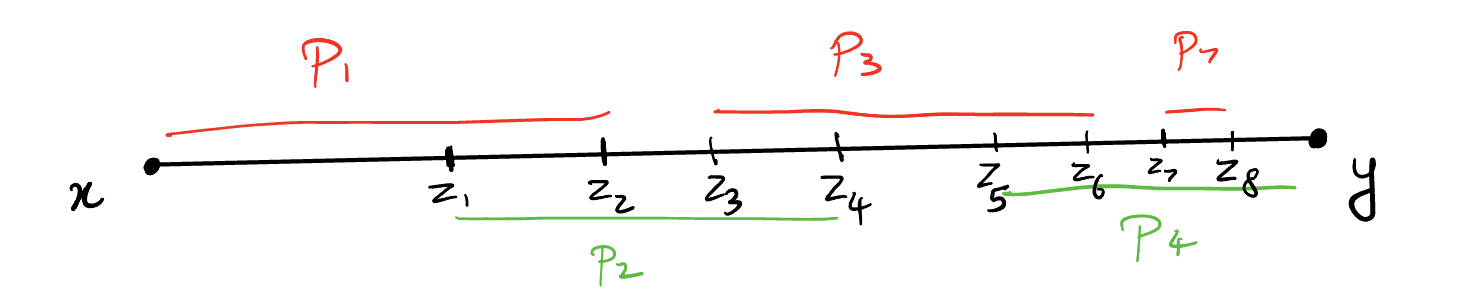
\includegraphics[scale=0.5]{images/schematic.png}
  \caption{A schematic of the geodesic $[x,y]$ traveling through several product regions.}
  \label{fig:schematic}
\end{figure}

Let $z_i$ denote the points on the geodesic segment that correspond to the times when the geodesic enters or exits a product region: in \autoref{fig:schematic}, we have labeled $z_i$ for $1 \leq i \leq 8$.
Let $\mathcal{J}_i$ denote the interval $[x, z_1]$ for $i=0$, the interval $[z_i, z_{i+1}]$ for $1 \leq i \leq 7$, and $[z_8, y]$ for $i=8$.
Let $\ell_i$ be the length of $\mathcal{J}_i$, and $e_i$ be the sum of the $h_i$ for each of the product regions that the interval $\mathcal{J}_i$ is in.
Also, for each $z_i$, let $z_i^{\prime}$ denote the nearest net point.

Keeping $x$ fixed, we can try to count the number of net points $y$ that satisfy the configuration we have described.
We have about $O(\exp(e_0 \ell_0))$ possibilities for $z_1^{\prime}$, and then keeping a $z_1^{\prime}$ fixed, $O(\exp(e_i \ell_1))$ possibilities for $z_2^{\prime}$ and so on.
Multiplying all these estimates, we have the following upper bound for cardinality of $y$.
\begin{align*}
  \#\left( y \right) \leq \exp\left( \sum_{i=0}^8 e_i \ell_i \right)
\end{align*}

The quantity $\sum e_i \ell_i$ serves as a re-weighted version of length of the geodesic in manner that works well with the counting function.
This is a primitive version of the \emph{complexity length} of $[x,y]$, and motivates the actual definition.

Before we define complexity length, we note two ways in which the above estimate overestimates the actual number of net points: that happens when a point in the geodesic is simultaneously in two or more product regions, which can happen in two ways.
\begin{enumerate}[(i)]
\item The product regions are disjoint: In this case, we are accounting the length of the geodesic segment multiple times: once for each product region we are in. However, this overcounting is still better than directly invoking Theorem \ref{thm:abem}, since the sums of the exponents $h_i$ associated to each of the disjoint product regions are smaller than the exponent associated to the entire surface.
\item The product regions are nested: In this case as well, we are accounting for the length of a geodesic multiple times, once for each product region we are in.
  Unlike in the previous case, in this case, the exponents associated to each product region can add up to a quantity larger than the exponent associated to the entire surface, which means the presence of nested product regions can give a worse estimate than Theorem \ref{thm:abem}.
  We will get around this problem by looking only at product regions associated to special subsurfaces which are called \emph{witnesses}.
\end{enumerate}

% Furthermore, a geodesic segment can enter and exit several product regions: in order to make the above analysis work in this more complicated setting, we will motivate and define \emph{complexity length} in the next subsection.

% The idea of complexity length is to assign to each point in a geodesic segment a weight which indicates the complexity of the product region that point in the geodesic is currently in.
% That means for a geodesic segment that lies entirely in the thick part, all of its points will be assigned weight equal to $6g-6 + 2b$.
% On the other hand, the geodesic segments in the above example will have all of their points assigned the weight $6g-6+2b-1$.
% \todo[inline]{Maybe make the above paragraph read slightly better.}

% For geodesic segments that enter and exit several product regions, assigning a weight to each point on the geodesic is a slightly more involved, and the content of the remainder of this section.

\subsection{An overview of complexity length}
\label{sec:an-overv-compl}

Now that we have motivated the need for complexity length, as well as considering special subsurfaces called witnesses, we formally define them in this section.
This section is a summary for Sections 7 through 12 of \textcite{dowdall2023lattice}, so we refer the reader to those sections for details we elide.
One difference in our presentation is that we care about these constructions for both orientable and non-orientable surfaces, while the original authors only work with orientable surfaces.
However, their constructions and proofs go through for non-orientable surfaces, as long as we provide a proof of the non-orientable versions of some of the foundational results they use.
We list those theorems here, and link to the proof of the non-orientable version that appears in Section \ref{sec:geom-of-teich}.
\begin{enumerate}[(i)]
\item Minsky's product region theorem (see Theorem \ref{thm:prno}).
\item Distance formula for Teichmüller space (see Theorem \ref{thm:distance-formula}).
\item Active intervals for subsurfaces (see Proposition \ref{thm:active-intervals}).
\item Consistency and realization (see Theorem \ref{thm:consistency-realization}).
\end{enumerate}

Let $\os$ be a surface (not necessarily orientable), and $\mathbf{C}$ some large arbitrary constant, and $\vept > 0$ a small constant we pick later.
We also pick constants $N_V$, for each $V \sqsubset \os$, such that $N_V$ only depends on the topological type of $V$.
The precise values of the $N_V$'s is specified via Proposition 10.13 of \cite{dowdall2023lattice}.
We will also abuse notation slightly and use $\hNP(V)$ to refer to $\hNP(\core(\teich(V)))$ whenever $V$ is a non-orientable surface: when $V$ is orientable, $\hNP(V)$ will refer to $\hNP(\teich(V))$.

Let $[x,y]$ be a geodesic segment in $\teich(\os)$: we describe the set of subsurfaces $\Upsilon(x, y)$ along which $[x, y]$ has large projections.
% \todo{Figure out the latex for the symbol Dowdall-Masur use for active subsurfaces.}

\begin{definition}[Active subsurfaces]
  A subsurface $V \sqsubset \os$ is an active subsurface, i.e. in $\Upsilon(x,y)$, if one of the following two conditions hold.
  \begin{enumerate}[(i)]
  \item The projection to $\cC(V)$ has diameter at least $N_V$.
  \item If $V$ is annular with core curve $\gamma$, then
    \begin{align*}
      \min\left( \ell_\gamma(x), \ell_{\gamma}(y) \right) < \vept
    \end{align*}
  \end{enumerate}
\end{definition}

Associated to each active subsurface $V$, there is a non-empty connected sub-interval of $[x,y]$, which we call an active interval, and denote $\mathcal{I}_V^{\vept}$, which we obtain via an application of Proposition \ref{thm:active-intervals}.
The active intervals associated to active subsurfaces enjoy the following properties.
\begin{enumerate}[(i)]
\item $\ell_\alpha(z) < \vept$ for $z \in \mathcal{I}_V^{\vept}$ and $\alpha \in \partial V$.
\item For $z \not \in \mathcal{I}_V^{\vept}$, $\ell_{\alpha}(z) > {\vept}^{\prime}$ for some $z \in \partial V$, and some ${\vept}^{\prime} < {\vept}$ that only depends on ${\vept}$.
\item For $[w,z] \subset [x,y]$ with $[w,z] \cap \mathcal{I}_V^{\vept} = \varnothing$, $d_V(w,z) \leq M_{\vept}$ for some $M_{\vept}$ that only depends on ${\vept}$.
\item For $U \pitchfork V$, $\mathcal{I}_U^{\vept} \cap \mathcal{I}_V^{\vept} = \varnothing$.
\end{enumerate}

For pairs of transverse subsurfaces $U \pitchfork V$, since $\mathcal{I}_U^{\vept} \cap \mathcal{I}_V^{\vept} = \varnothing$ we can also determine which of the subsurfaces are active first.
\begin{definition}[Behrstock partial order]
  If $U$ and $V$ are a pair of transverse subsurfaces in $\Upsilon(x,y)$, we say $U \lessdot V$ if $\mathcal{I}_U^{\vept}$ appears to the left of $\mathcal{I}_V^{\vept}$ in $[x,y]$.
\end{definition}

Observe that when restricted to $\mathcal{I}_V^{\vept}$, the geodesic is traveling in a product region, one of whose components is $\teich(V)$, but trying to apply the technique from the previous subsection leads to the problem of overcounting, namely overcounting arising from subsurfaces either nested in $V$, or subsurfaces $V$ is nested in.

To deal with this issue, we will consider a subset of $\Upsilon(x,y)$, called a \emph{witness family}.
However, to avoid overcounting, some additional properties are required of the witness families.
Rather than defining all of those properties without context, we introduce them one at a time, after motivating the need for the property.

\begin{definition}[Witness family]
  A witness family $\Omega(x,y)$ associated to the geodesic $[x,y]$ is a subset of $\Upsilon(x, y)$ satisfying the following properties.
  \begin{enumerate}[(i)]
  \item For any $Z \in \Upsilon(x,y)$, $Z \sqsubset W$ for some $W \in \Omega(x,y)$.
  \item If $Z \sqsubset W$, and $Z \in \Omega(x,y)$ and $W \in \Upsilon(x,y)$, then $W$ must also either be a witness, or must be transverse to a witness $V \in \Omega(x,y)$ such that $Z \sqsubset V$.
  \end{enumerate}
\end{definition}
The first condition of the definition ensures that when we restrict our attention from all active subsurfaces to witnesses, we do not lose information, i.e. every active subsurface contributes to whichever witness it is contained in.
The second condition is a more technical requirement that is required to ensure that the other properties we define later work nicely.
% {\color{red} The second condition is a more technical requirement that we will motivate later.}

We now make the notion of an active subsurface \emph{contributing to a witness} more precise.
\begin{definition}[Complete witness family]
  For an active subsurface $V$, a witness $W$ is said to be the $\Omega$-completion of $V$, denoted $\colsup{V}{\Omega}$ if $W$ is the minimal (by inclusion) witness containing $V$.
  If $W = \colsup{V}{\Omega}$, we say $V$ \emph{contributes} to $W$.
  Furthermore, a witness family is \emph{complete} if every active subsurface has a unique $\Omega$-completion.
\end{definition}

By partitioning off the collection active subsurfaces into classes, where each class is represented by a witness, and only considering the product regions associated to the witnesses, rather than all the active subsurfaces, we can cut down on the overcount we obtain by considering all active subsurfaces.

We now look at an extreme example of a complete witness families to motivate further properties that we will need from the witness families in order to count well.

\begin{example}[Trivial witness family]
  \label{ex:uninsulated}
  Let $\gamma$ be a pseudo-Anosov mapping class on $\os$, such that $\gamma$ has large translation distance on $\cC(\os)$, and $\delta$ a reducible mapping class, acting on a subsurface $V$ such that the action of $\delta$ on $\cC(V)$ has large translation distance as well.

  Let $x$ be a point in $\teich(\os)$, and $y = \delta \gamma \delta^{-1} x$.
  The active subsurfaces for $[x, y]$ contain the surfaces $\os$, $V$, and $\gamma V$: however, we can pick $\Omega(x,y) = \left\{ \os \right\}$, and check that this is a complete witness family.
\end{example}

  In the above example, since we only have one subsurface in our witness family, we certainly don't overcount via overlapping product regions, but we do end up ignoring the fact that the geodesic $[x,y]$ travels in a smaller product region near the beginning of the segment, as well as the end.
  For the initial and the final segment of the geodesic, the witness $\os$ is too big for the subsurface the geodesic is actually traveling in.
  This suggest that a better choice of a witness family would be to include both $V$ and $\gamma V$ as witnesses too.
  We can take this approach further, and include every subsurface in $\Upsilon(x,y)$ as a witness: this will still form a complete witness family.
  However, this approach also leads to multiple witnesses nested within one another, which is something we want to avoid as much as possible.

  The drawback of Example \ref{ex:uninsulated} motivates the next property we will require from witness families, which is the notion of being \emph{insulated}.
  Informally, a witness family $\Omega(x,y)$ is insulated if all the maximal active subsurfaces that are active near the beginning or end of $[x,y]$ are also witnesses.
  \begin{definition}[Insulated witness family]
    \label{def:insulated}
    A witness family $\Omega(x,y)$ is insulated if for every $E \in \Omega(x,y)$, the following subsurfaces $V \sqsubset E$ are also witnesses.
    \begin{enumerate}[(i)]
    \item $V \in \Upsilon(x,y)$.
    \item $d_E(\cC(V), x) \leq 9\mathbf{C}$, or $d_E(\cC(V), y) \leq 9 \mathbf{C}$, where we consider $\cC(V)$ to be a subset of $\cC(E)$.
    \item $V$ is topologically maximal among the subsurfaces that satisfy (i) and (ii).
    \end{enumerate}
  \end{definition}

  % A benefit of co
  Once we have an insulated witness family, we can order a nested pair of witnesses $W \sqsubset V$ based on whether $W$ is active near the beginning or the end of the geodesic $[x,y]$ projected to $\cC(V)$.

  \begin{definition}[Subordering]
    Let $[x,y]$ be a geodesic in $\teich(\os)$ and $\Omega(x,y)$ a complete insulated witness family associated to $[x,y]$.
    Then for each nested pair of witnesses $W \sqsubset V$, a subordering is an assignment of exactly one of the following two possibilities:
    \begin{enumerate}[(i)]
    \item $W \swarrow V$
    \item $V \searrow W$
    \end{enumerate}
    The orderings $\swarrow$ and $\searrow$ satisfy the following properties.
    \begin{enumerate}[(i)]
    \item If $Z$, $V$, and $W$ are witnesses such that $Z \sqsubset V \sqsubset W$, then $Z \swarrow W$ iff $V \swarrow W$ (equivalently, $W \searrow Z$ iff $W \searrow V$).
    \item If $Z$, $V$ and $W$ are witnesses such that $Z \swarrow V \searrow W$, then $Z \pitchfork_V W$ and $Z \lessdot W$.
    \item If $Z$ and $V$ are witnesses, and $W$ an active subsurface such that $Z \swarrow V \lessdot W$, or $W \lessdot V \searrow Z$, then $Z \pitchfork_V W$.
    \item If $Z$ and $V$ are witnesses, such that $Z \swarrow V$ (or $Z \searrow V$), then there does not exist any active subsurface $W$ such that the $\Omega$-closure of $W$ is $V$ and $W \lessdot V$ (or $V \lessdot W$).
    \end{enumerate}
  \end{definition}

  We now provide some motivation for the various conditions that appear in the above definition.
  First of all, when we see $Z \swarrow W$, we are to read that as \emph{the geodesic $[x,y]$ makes progress in the nested subsurface $Z$, before making progress in the supersurface $W$}.
  Similarly, when we see $W \searrow Z$, we are to read that as \emph{the geodesic $[x,y]$ make progress in the supersurface $W$ before making progress in the nested subsurface $Z$}.
  With this description of the subordering, conditions (i) and (iv) of the definition are easy to understand. The conditions (ii) and (iii) let us upgrade $\swarrow$ and $\searrow$ to transversality and time-ordering.
  A more intuitive reading of condition (ii) for instance would be, if $Z swarrow V \searrow W$, that means the geodesic makes progress in $Z$ before $V$, and then makes progress in $W$.
  That means if we just look at $V$ and $W$, it makes progress in $V$ and then $W$. And since neither of them are nested in the other, the only way they can be time-ordered is by being transverse relative to $V$.

  We can also see how the subordering on a witness family interacts with the witness family being insulated: recall the pair of witnesses $V \sqsubset E$ from Definition \ref{def:insulated}.
  \begin{itemize}
  \item If $d_E(\cC(V), x) \leq 9 \mathbf{C}$, then $V \swarrow E$, since the geodesic makes progress in $V$ before $E$.
  \item If $d_E(\cC(V), Y) \leq 9 \mathbf{C}$, then $E \searrow V$, since the geodesic makes progress in $E$ before $V$.
  \end{itemize}
  However, the above example does not capture all the ways in which we can have $V \swarrow E$ or $E \searrow V$.
  Consider a decomposition of a Teichmüller geodesic by the active intervals corresponding to witnesses illustrated in \autoref{fig:subordering-examples}.
  \begin{figure}[h]
    \centering
    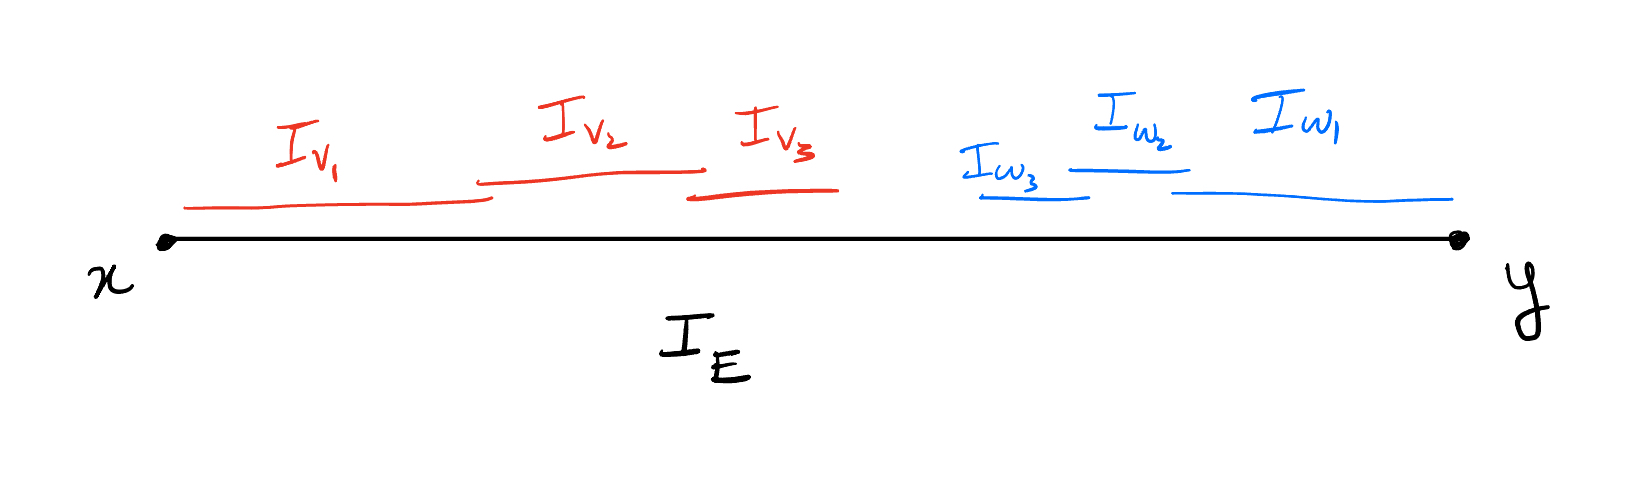
\includegraphics[scale=0.5]{images/subordering-example.png}
    \caption{Examples of $V_i \swarrow E$ and $E \searrow W_i$.}
    \label{fig:subordering-examples}
  \end{figure}

  In this example, all of the witnesses $V_i$ satisfy $V_i \swarrow E$, and all of the witnesses $W_i$ satisfy $E \searrow W_i$, but $d_E(\cC(V_i), x)$ need not be less than $9\mathbf{C}$ for $i=2$ or $i=3$, and similarly, $d_E(\cC(W_i), y)$ need not be less than $9 \mathbf{C}$ for $i=2$ or $i=3$.

  In fact, the above example illustrates that for witnesses $V$ that are not within distance $9 \mathbf{C}$ from one of the endpoints, the choice between assigning $V \swarrow E$ and $E \searrow V$ is ambiguous, which is what the property of being \emph{wide} tries to fix.
  The property of being \emph{wide} also tells when an active subsurface $V$ nested in a witness $E$ contributes to $E$: this happens when $V$ appears in the ``middle'' of the segment $[x,y]$.

  % \todo[inline]{Specify that this definition needs ISC witness families}

  \begin{definition}[Wide witness families]
    An insulated complete subordered witness family is wide if for each $V$ in the witness family, both of the following quantities are at most $\frac{N_V}{3}$.
    \begin{itemize}
    \item For $W$ a witness such that $W \swarrow V$, the quantity $\mathrm{diam}_V(x, \cC(W))$.
    \item For $W$ a witness such that $V \searrow W$, the quantity $\mathrm{diam}_V(y, \cC(W))$.
    \end{itemize}
  \end{definition}

  The idea behind a wide witness family is to create a buffer zone of length at least $\frac{N_V}{3}$ in the middle of the projection of the geodesic to $\cC(V)$ for any witness $V$ such that:
  \begin{itemize}
  \item If any subsurface $W$ is active to the left of the buffer zone, it contributes to a subsurface $Z$ such that $Z \swarrow V$.
  \item If any subsurface $W$ is active to the right of the buffer zone, it contributes to a subsurface $Z$ such that $V \searrow Z$.
  \item If a subsurface $W$ is active within the buffer zone, it contributes to $V$.
  \end{itemize}

  The upshot of defining wide, insulated, subordered, and complete witness families (which will be abbreviated to WISC witness families) is that it gives us a better idea the order in which progress is made in various active subsurfaces.
  If we were working with just the collection of active subsurfaces, the only time we can tell if a geodesic makes progress in a subsurface $V$ followed by the subsurface $W$ is when $V \pitchfork W$.
  When working with a WISC witness family, we can do that, but we can also make similar statements about pairs of nested witnesses $V \sqsubset W$, namely we can have either $V \swarrow W$ or $W \searrow V$.

  The following lemma asserts that WISC witness families exist, and their cardinality can be uniformly bounded.
  \begin{lemma}[Lemmas 7.29 and 7.30 from \cite{dowdall2023lattice}]
    Let $\os$ be surface, and $[x,y]$ a geodesic segment in $\teich(\os)$.
    Then there exists a WISC witness family $\Omega(x,y)$ for $[x,y]$.
    Furthermore, the cardinality of $\Omega(x,y)$ depends only on $\os$, and not the points $x$ and $y$.
  \end{lemma}
  \begin{rem}
    While the statements of Lemmas 7.29 and 7.30 in \textcite{dowdall2023lattice} are for orientable surfaces, they go through without any changes for non-orientable surfaces as well.
  \end{rem}

  We now get to the raison d'\^etre of witness families: turning points on the geodesic segment $[x,y]$ in $\teich(\os)$ into points in $\teich(V)$, where $V$ is a witness in $\Omega(x,y)$.
  We will do so by assigning to each point $w$ in a neighbourhood of $[x,y]$ a point $\wt{w}_Z$ in $\cC(Z)$ for all subsurfaces $Z$ contained in $V$, and then showing this assignment is consistent.
  Then the realization theorem (Theorem \ref{thm:consistency-realization}) will give us a point $\widehat{w}_V^{\Omega}$ in $\teich(V)$ which has the same projections in $\cC(Z)$ as the original point $W$.
  \begin{definition}[Projection tuple]
    \label{def:projection-tuple}
    Let $\Omega(x,y)$ be a WISC witness family for a Teichmüller geodesic $[x,y]$ in $\teich(\os)$.
    Let $w$ be a point in $\teich(\os)$ satisfying the following bound for every active subsurface $V$.
    \begin{align*}
      d_{V}(x, w) + d_{V}(w, y) \leq d_{V}(x, y) + 9 \mathbf{C}
    \end{align*}
    Then for any $U \in \Omega(x,y)$, the projection tuple $\wt{w}$ of $w$ is the point in $\prod_{Z \sqsubseteq U} \cC(Z)$ given by the following formula (where $\pi_Z$ is the usual projection map from $\teich(\os)$ to $\cC(Z)$).
    \begin{align*}
      \wt{w}_Z =
      \begin{cases}
        \pi_Z(y), & \text{if $Z \in \Upsilon(x,y)$ and $\colsup{Z}{\Omega} \swarrow U$} \\
        \pi_Z(x), & \text{if $Z \in \Upsilon(x,y)$ and $U \searrow \colsup{Z}{\Omega}$} \\
        \pi_Z(w), & \text{otherwise}
      \end{cases}
    \end{align*}
  \end{definition}

  Observe that this is different from the usual projection map from $\teich(\os)$ to $\cC(Z)$: for subsurfaces $Z$ that contribute to a witness nested in $U$, and consequently, $\colsup{Z}{\Omega} \swarrow U$ or $U \searrow \colsup{Z}{\Omega}$, we change the projection from $\pi_Z(w)$ to $\pi_Z(y)$ or $\pi_Z(x)$ respectively.
  % \todo[inline]{Motivate the reason for this modified projection map?}

  This new projection map, despite being a modification of the usual projection map, is still consistent.
  \begin{proposition}[Proposition 8.4 of \cite{dowdall2023lattice}]
    The projection tuple $\wt{w}_Z$ is $k$-consistent for some $k$ depending only on $\mathbf{C}$.
  \end{proposition}

  Using the above proposition, and the realization theorem for non-orientable surfaces (Theorem \ref{thm:consistency-realization}), we can turn a projection tuple into a point in $\teich(U)$, which \textcite{dowdall2023lattice} refer to as \emph{resolving a point $w$ in $\teich(U)$}.
  \begin{definition}[Resolution point]
    Let $[x,y]$ be a geodesic segment in $\teich(\os)$, and $\Omega(x,y)$ an associated WISC witness family.
    For $w \in \left\{ x, y \right\}$, and $U \in \Omega(x,y)$, we define $\widehat{w}_U^{\Omega}$ as follows.
    \begin{itemize}
    \item If $U$ is non-annular, then $\widehat{w}_U^{\Omega} \in \teich(U)$ is the thick point whose projections to $\cC(V)$ for $V \sqsubseteq U$ are coarsely equal to the projection tuple $\widehat{w}_U$ (which exists due to the Realization theorem (Theorem \ref{thm:consistency-realization})).
    \item If $U$ is annular, then $\wt{w}_U$ is an element of $\mathbb{Z}$, and we set $\widehat{w}_U^{\Omega}$ to be the point in $\mathbb{H}$ whose twist coordinate is $\wt{w}_U$, and whose length coordinate is $\displaystyle \frac{1}{\min\left( {\vept}, \ell_{\partial U}(w) \right)}$.
    \end{itemize}
  \end{definition}

  We can now define the complexity length associated to a witness family $\Omega$.

  \begin{definition}[Complexity of witness family]
    Let $[x, y]$ be a geodesic segment in $\teich(\os)$, and $\Omega$ an associated WISC witness family.
    The complexity $\mathfrak{L}_{\Omega}(x,y)$ of $\Omega$ is the following quantity.
    \begin{align*}
      \mathfrak{L}_{\Omega}(x,y) \coloneqq \sum_{U \in \Omega} \hNP^{\ast}(U) \cdot d_{\teich(U)}(\widehat{x}_{U}^{\Omega}, \widehat{y}_{U}^{\Omega})
    \end{align*}
    Here, $\hNP^{\ast}(U)$ is the net point growth entropy for $\teich(U)$ when $U$ is non-annular, and when $U$ is annular, $\hNP^{\ast}(U)$ is $1$ when both $\widehat{x}_{U}^{\Omega}$ and $\widehat{y}_{U}^{\Omega}$ are ${\vept}$-thick, and $2$ if not.
  \end{definition}

We now address why we used a modified version of the projection map in Definition \ref{def:projection-tuple} instead of the usual projection map to curve complexes, by revisiting Example \ref{ex:uninsulated}.
\begin{example}
  \label{ex:need-for-modified-projection}
  Let $\gamma$ be a pseudo-Anosov mapping class on $\os$, with large translation distance on $\cC(\os)$ and small projections elsewhere.
  Let $\delta$ be a reducible mapping class, which is psuedo-Anosov on a subsurface $V$, with large translation distance on $\cC(V)$ and small translation distance everywhere.
  Let $x$ be a point in $\teich(\os)$, and $y = \delta \gamma \delta^{-1} x$.
  We first verify that $\Upsilon(x,y) = \left\{ \os, V, \delta \gamma V \right\}$.
  To see this, we consider the following tuple of points $(x, \delta x, \delta \gamma x, \delta \gamma \delta^{-1}x)$.
  We claim that each of the points in the tuple lies coarsely on the geodesic $[x,y]$, and computing the projections of adjacent pairs of points in tuple, we get the following.
  \begin{itemize}
  \item[-] $[x, \delta x]$ has large projections on $\cC(V)$ and small projections on other curve complexes.
  \item[-] $[\delta x, \delta \gamma x]$ has large projections on the $\cC(\delta \os)$, which is the same as $\cC(\os)$, and small projections elsewhere.
  \item[-] $[\delta \gamma x, \delta \gamma \delta^{-1} x]$ has large projections on $\cC(\delta \gamma V)$, and small projections elsewhere.
  \end{itemize}
  Let $\Omega(x, y) = \Upsilon(x,y) = \left\{ \os, V, \delta \gamma V \right\}$.
  % \todo[inline]{Add more details about why $\delta \gamma V$ is the correct domain.}
  One can verify that this is a WISC witness family for $[x,y]$.
  Furthermore, we have that $V \swarrow \os$ and $\os \searrow \gamma V$.

  We now compute the resolution of the points $x$ and $y$ in $\teich(V)$, $\teich(\gamma V)$, and $\teich(\os)$.
  Observe that the geodesic $[x,y]$ almost immediately moves into a product region associated to $V$ at the beginning, leaves that product region at some point $w$ along the geodesic, and then enters the product region associated to $\gamma V$ at some point $z$, and then stays in that product region almost all the way up to the end.
  We will abuse notation slightly, and refer to $x$ and $w$ as points in $\teich(V)$, when we mean their projection via the product region map, and $z$ and $y$ will refer to points in $\teich(\gamma V)$
  Resolving points in $\teich(V)$ and $\teich(\gamma V)$ is easy, since there's no other witnesses nested in them, which means the projection tuple for those subsurfaces is the usual projection map.
  \begin{align*}
    \widehat{x}_V^{\Omega} &= x \\
    \widehat{y}_V^{\Omega} &= w \\
    \widehat{x}_{\gamma V}^{\Omega} &= z \\
    \widehat{y}_{\gamma V}^{\Omega} &= y \\
  \end{align*}
  To resolve points in $\teich(\os)$, we have to use our modified projection map, instead of the usual one.
  Doing so, the points $x$ and $y$ resolve in the following manner.
  \begin{align*}
    \widehat{x}_{\os}^{\Omega} = w \\
    \widehat{y}_{\os}^{\Omega} = z
  \end{align*}

  If we instead used the usual projection maps, $\widehat{x}_{\os}^{\Omega}$ would resolve to $x$, and $\widehat{y}_{\os}^{\Omega}$ would resolve to $y$.
  Consequently, we would not have the following estimate for complexity in terms of Teichmüller distance.
  \begin{align*}
    \mathfrak{L}_{\Omega}(x,y) &= \hNP^{\ast}(V) \cdot d_{\teich(V)}(x, w) + \hNP^{\ast}(\os) \cdot d_{\teich(\os)}(w, z) + \hNP^{\ast}(\gamma V) \cdot d_{\teich(\gamma V)}(z, y) \\
    &< \hNP^{\ast}(\os) \cdot d_{\teich(\os)}(x, y)
  \end{align*}
\end{example}

Constructing the resolution points $\widehat{x}_V^{\Omega}$ and $\widehat{x}_V^{\Omega}$ via the Realization theorem does not provide us very good bounds for $d_{\teich(V)}(\widehat{x}_V^{\Omega}, \widehat{x}_V^{\Omega})$.
At best, we accrue multiplicative and additive errors if we use Rafi's distance formula to estimate this distance from the curve complex distances.
For our applications however, the most we can tolerate is additive error.
To do this, we will need to refine to notion of active interval for a subsurface to something more useful for the estimate: the \emph{contribution set} $\mathcal{A}_V^{\Omega}$ of a witness $V$.
We first define two intermediate collections of subintervals of a geodesic segment $[x,y]$.
\begin{align*}
  M(V) &\coloneqq \bigcup \left\{ \mathcal{I}_W^{{\vept}} \mid \text{$W \in \Omega$ with $W \sqsubset V$ }  \right\} \\
  C(V) &\coloneqq \bigcup \left\{ \mathcal{I}_Z^{{\vept}} \mid \text{$Z$ contributes to $V$} \right\}
\end{align*}

\begin{definition}[Contribution set]
  For a witness $V \in \Omega$, the contribution set $\mathcal{A}_V^{\Omega}$ is a subset of the geodesic segment $[x,y]$ defined in the following manner.
  \begin{align*}
    \mathcal{A}_V^{\Omega} \coloneqq \left( \mathcal{I}_V^{\vept} \setminus M(V) \right) \cup C(V)
  \end{align*}
\end{definition}
\begin{rem}
  The reason we remove $M(V)$ and then later add $C(V)$ again is because it is possible for several different subsurfaces to be active at the same time: orthogonal subsurfaces for instance.
  One can have $V$ and $W$ as witnesses, with $W \sqsubset V$, and $Z \sqsubset V$ an active subsurface but not a witness, such that $W \perp Z$ with $\mathcal{I}_W^{\vept}$ and $\mathcal{I}_Z^{\vept}$ overlapping.
  In that case, removing $M(V)$ would also remove part of $\mathcal{I}_Z^{\vept}$, and adding back $C(V)$ would add back the deleted portion.
\end{rem}

The following theorem estimates $d_{\teich(V)}(\widehat{x}_V^{\Omega}, \widehat{y}_V^{\Omega})$ using $\mathcal{A}_V^{\Omega}$.
\begin{theorem}[Theorem 9.4 of \cite{dowdall2023lattice}]
  \label{thm:contribution-set-resolution-distance}
  There exists a uniform constant $C$ such that the following bound holds for any $x$, $y$, and witness $V$.
  \begin{align*}
d_{\teich(V)}(\widehat{x}_V^{\Omega}, \widehat{y}_V^{\Omega}) \leq \int_x^y \mathbbm{1}_{\mathcal{A}_V^{\Omega}} + C
  \end{align*}
\end{theorem}

Contribution sets help us make precise the notion of ``overcounting'' when multiple product regions are active at the same time.
More precisely, when a segment of $[x,y]$ is a part of two or more contribution sets, that segment shows up multiple times when computing $\mathfrak{L}_{\Omega}(x,y)$, thanks to Theorem \ref{thm:contribution-set-resolution-distance}.
If the overlapping segment is sufficiently long, one could even end up having $\mathfrak{L}_{\Omega}(x,y) > \hNP^\ast(\os) \cdot d_{\teich(\os)}(x, y)$, which as we will see, leads to a worse count for net points than the usual methods.
This phenomenon of contribution sets overlapping is called \emph{badness}, and while we will not be able to eliminate it entirely, we will be able to minimize it.

\begin{definition}[Bad set]
  We say a point $p$ in $\mathcal{A}_V^{\Omega}$ is bad if there exists some other witness $W$ such that $p$ also belongs in $\mathcal{A}_W^{\Omega}$.
  The bad set $\mathcal{B}_V^{\Omega}$ denotes the set of all bad points in $\mathcal{A}_V^{\Omega}$, and $\left| \mathcal{B}_V^{\Omega} \right|$ denotes the total length of this set, when we think of $\mathcal{B}_V^{\Omega}$ as a subset of the geodesic segment $[x,y]$.
\end{definition}

For our applications, we won't need to eliminate badness entirely, or even bound the length of the bad set uniformly: it will suffice to show that the length of the bad set is a very small multiple of $d_{\teich(\os)}(x,y)$.

\begin{definition}[Admissible and limited]
  A witness family $\Omega$ associated to a geodesic segment $[x,y]$ is said to be:
  \begin{itemize}
  \item \emph{admissible} if $\displaystyle \left| \mathcal{B}_V^{\Omega} \right| \leq \frac{d_{\teich(\os)}(x,y)}{K_V \mathbf{C}}$, for all $V \in \Omega$, and some constants $K_V$ that only depend on the topological type of $V$.
  \item \emph{limited} if $\left| \Omega \right|$ is uniformly bounded, independent of $x$ and $y$.
  \end{itemize}
\end{definition}
\begin{rem}
  Our definition of limited is a weaker version of Definition 10.7 from \textcite{dowdall2023lattice}, but since we don't need the stronger version, we present this version instead.
\end{rem}

\textcite{dowdall2023lattice} prove that WISC witness families that are admissible and limited exist. They call these witness families WISCAL witness families.

\begin{proposition}[Section 10.3 of \cite{dowdall2023lattice}]
  For all $[x,y]$, there exists an associated WISC witness family that is also admissible and limited.
\end{proposition}

For WISCAL witness families, the following result relating complexity and Teichmüller distance follows easily from Theorem \ref{thm:contribution-set-resolution-distance} and the definition of admissible.

\begin{proposition}
  \label{prop:complexity-length-inequality}
  If $\Omega$ is a WISCAL witness family associated to $[x,y]$, then the following inequality holds.
  \begin{align*}
    \mathfrak{L}_{\Omega}(x,y) \leq \left( \hNP(\os) + \frac{K}{\mathbf{C}} \right) d_{\teich(\os)}(x, y) + K \mathbf{C}
  \end{align*}
  Here, $K$ is some uniform constant depending only on $\os$.
\end{proposition}

% For triples of points that do not backtrack, there exists a version of the above inequality similar to a reverse triangle inequality.

% \begin{definition}[$\theta$-aligned]
%   A triple of points $(x,y,z)$ in $\teich(\os)$ is said to be $\theta$-aligned if the following inequality holds for all subsurfaces $V$.
%   \begin{align*}
%     d_V(x, y) + d_V(y, z) \leq d_V(x, z) + \theta
%   \end{align*}
% \end{definition}

% \begin{theorem}[Theorem 11.2 of \cite{dowdall2023lattice}]
%   If $(x, y, z)$ is a $\mathbf{C}$-aligned triple in $\teich(\os)$, and $\Omega_1$ is a WISCAL witness family for $[x,y]$, and $\Omega_2$ a WISCAL witness family for $[y,z]$, then the following inequality holds.
%   \begin{align*}
%     \mathfrak{L}_{\Omega_1}(x, y) + \mathfrak{L}_{\Omega_2}(y, z) \leq \left( \hNP(\os) + \frac{K}{\mathbf{C}} \right) d_{\teich(\os)}(x,z) + K \mathbf{C}
%   \end{align*}
%   Here, $K$ is some uniform constant depending only on $\os$.
% \end{theorem}

We now define complexity length, which follows from the definition of the complexity of a witness family.

\begin{definition}[Complexity length]
  \label{defn:complexity-length}
  For a pair of points $x$ and $y$ in $\teich(\os)$, the complexity length $\mathfrak{L}(x,y)$ is defined to be the following.
  \begin{align*}
    \mathfrak{L}(x,y) \coloneqq \inf_{\Omega} \mathfrak{L}_{\Omega}(x,y)
  \end{align*}
  Here, we take the infimum over all WISCAL witness families for $[x,y]$.
\end{definition}

With the machinery of complexity length set up, it is now possible to count net points with respect to complexity length.

\begin{theorem}[Theorem 12.1 of \cite{dowdall2023lattice}]
  \label{thm:counting-with-complexity}
  For any large enough $\mathbf{C} > 0$, and any $\veperr > 0$, there exists an polynomial function $p(r)$, and $r > 0$ large enough such that the following bound holds for net points in $\teich(\os)$.
  \begin{align*}
    \# \left( y \in \net \mid \mathfrak{L}(x,y) \leq r \right) \leq p(r) \cdot \exp\left( (1+\veperr)r \right)
  \end{align*}
\end{theorem}
%\todo[inline]{Make sure we're using consistent notation for net.}

\begin{rem}
  The above theorem is a slightly weaker version of the theorem that appears in \textcite{dowdall2023lattice}: their version does not have the $\veperr$.
  The reason we have the weaker version is that in the proof of their theorem, they count the number of net points in $\teich(V)$ in a ball of radius $R$, where $V$ is a witness, using Theorem \ref{thm:abem}, which gives them that the number of net points is equal, up to multiplicative error, to $\exp(\hNP(U) R)$.
  Since Theorem \ref{thm:abem} only holds orientable surfaces, and we want to state our results for non-orientable surfaces as well, we will need to use a weaker counting result to count net points in $\teich(V)$, namely the following bound, which holds for any $\vepent > 0$ and large enough $R$.
  \begin{align*}
    \#\left( y \in \net \mid d_{\teich(V)}(x, y) \leq R \right) \leq \exp\left( (\hNP(V) + \vepent ) R \right)
  \end{align*}
\end{rem}

We sketch out a proof of Theorem \ref{thm:counting-with-complexity} below: the proof proceeds identically to the proof in \textcite{dowdall2023lattice}, except at one point, where we plug in our weaker bound for net points in $\teich(V)$ for witnesses $V$.

\begin{proof}[Sketch of proof for Theorem \ref{thm:counting-with-complexity}]
  For each $y \in \net$ such that $\mathfrak{L}(x,y) \leq r$, we have a WISCAL witness family $\Omega$ such that $\mathfrak{L}_{\Omega}(x,y) \leq r$.
  We can turn that witness family into a graph in the following manner.
  \begin{itemize}
  \item Add a vertex for every witness $V \in \Omega$.
  \item Label the vertex associated with $V$ with the tuple $(\hNP^{\ast}(V), \lfloor d_{\teich(V)}(\widehat{x}_{V}^{\Omega}, \widehat{y}_{V}^{\Omega}) \rfloor)$.
  \item If we have a pair of witnesses $V \swarrow W$, we join the vertices associated to them with a directed edge labeled ``SW'': $V \xrightarrow{SW} W$.
  \item If we have a pair of witnesses $W \searrow V$, we join the vertices associated to them with a directed edge labeled ``SE'': $W \xrightarrow{SE} V$.
  \item If we have a pair of witnesses $W \pitchfork V$, with $W \lessdot V$, we join the vertices associated to them with a directed edge labelled ``P'': $W \xrightarrow{P} V$.
  \end{itemize}

  We first count how many distinct possibilities are there for such labeled graphs that correspond to $y$ for which $\mathfrak{L}(x,y) \leq r$.
  Since the cardinality of a WISCAL family is uniformly bounded, there are at most $k$ many vertices, for some constant $k$.
  As for the labels on the vertices, there are at most $\frac{r}{\hNP^{\ast}(V)}$ possibilities for a label on vertex which corresponds to a subsurface which is homeomorphic to $V$.
  From this, we conclude that there are at most $p(r)$ possibilities for the combinatorial type of the graph, where $p(r)$ is a polynomial in $r$.

  It will suffice to compute how many distinct net points give rise to witness families whose graph is of a given type.
  To do so, we consider \emph{initial subsets} of the graph, i.e. a subset $\mathcal{W}$ of the vertices $\mathcal{V}$ of the graph such that there is no directed edge from $\mathcal{V} \setminus \mathcal{W}$ to $\mathcal{W}$.

  Given an initial subset $\mathcal{W}$ of the graph, we construct points $y$ such that the witness family associated to $[x,y]$ has the combinatorial type $\mathcal{W}$.
  We then consider an enlargement of $\mathcal{W}$ by one-additional vertex $v$, such that the enlargement is still an initial subset.
  \begin{claim*}
    The entire graph $\mathcal{V}$ can be built up from such one-step enlargements.
  \end{claim*}

  We then count the number of net points whose associated witness families have the combinatorial type $\mathcal{W} \cup \left\{ v \right\}$, after we fix one witness family associated to $\mathcal{W}$.
  More concretely, let $w$ be a point such that the combinatorial type of the witness family associated to $[x,w]$ is $\mathcal{W}$.
  Suppose now that we add a vertex $(h, r_0)$ to the graph $\mathcal{W}$.
  To extend $\Omega(x,w)$ so that its combinatorial type is $\mathcal{W} \cup \left\{ (h, r_0) \right\}$, we need to add a witness $U$ whose net point entropy is $h$, and travel for distance $r_0$ in the Teichmüller space of $U$.
  There are only finitely many choices for such subsurfaces $U$ (because their boundary curves must get short near $w$), and once we've made a choice of $U$, we have a choice $\exp\left( (\hNP(V) + \vepent) r_0 \right)$ points.

  Multiplying out the counts for each vertex added, we get the following estimate for the cardinality associated to each combinatorial type.
  \begin{align*}
    \#\left( y \mid \text{$\Omega(x,y)$ has combinatorial type $\mathcal{V}$} \right) &= \sum_{(h, s) \in \mathcal{V}} \exp\left( (h + \vepent)s \right) \\
    &\leq \exp\left( (1 + \veperr)r \right)
  \end{align*}
  We get the second inequality by picking $\vepent$ small enough, and observing that $\sum hs = r$.
\end{proof}

\subsection{Linear gap for bad points}
\label{sec:linear-gap-bad}

In this subsection, we will prove our main result involving complexity length: on the complexity length of bad points.

\begin{theorem}
  \label{thm:linear-gap}
  Suppose that for all proper subsurfaces $V$ of $\os$, the following inequality holds.
  \begin{align*}
    \hNP(V) < \hNP(\os)
  \end{align*}
  Then for any $\vepb > 0$, there exists $c > 0$, and $R$ large enough, such that for any bad point $y$, i.e. a point in $\net_b(p, R, \vepb)$, the following upper bound holds for the complexity length between $p$ and $y$.
  \begin{align*}
    \mathfrak{L}(p, y) \leq \hNP(\os) (1 - c) R
  \end{align*}
\end{theorem}

\begin{proof}


Let $\Omega$ be a WISCAL witness family for $[p, y]$: the proof of Theorem \ref{thm:linear-gap} splits into two cases depending on whether the surface $\os$ is a witness in $\Omega$ or not.

The former case is harder, so we deal with that first.
% \begin{lemma}
%   The triple $(p, \widehat{y}_{\os}^{\Omega}, y)$ is $\theta$-aligned, for some constant $\theta$ independent of $R$ and $y$.
% \end{lemma}

% \begin{proof}
%   Recall that we define $\widehat{y}_{\os}^{\Omega}$ by specifying its coordinates in the curve complex of a subsurface $V$ according to the following rule.
%   \begin{itemize}
%   \item $\pi_V(y)$ if $\overline{V} \swarrow \os$.
%   \item $\pi_V(p)$ if $\os \searrow \overline{V}$.
%   \item $\pi_V(y)$ otherwise.
%   \end{itemize}
%   In all of these cases, the resulting triple in $\cC(V)$ looks like $(p,p,y)$ or $(p,y,y)$, which are trivially $\theta$-aligned for some uniform constant $\theta$.
% \end{proof}

We consider the triple of points $(p, \widehat{y}_{\os}^{\Omega}, y)$, and first estimate $\mathfrak{L}(p, \widehat{y}_{\os}^{\Omega})$.
% Observe that from the way we have defined $\widehat{y}_{\os}^{\Omega}$, it's within a bounded distance of the point $q$ on $[p,y]$ which is the last point on $[p, y]$ which stays in the thick part.

% By hypothesis of $y$ being a bad point, we have the following bounds on Teichmüller distance.
% \begin{align*}
%   % d_{\teich(\os)}(q, y) &> \vepb R \\
%   d_{\teich(\os)}(p, q) &\leq (1-\vepb) R
% \end{align*}
% Since $\widehat{y}_{\os}^{\Omega}$ is within bounded distance of $q$, we get similar bounds for $\widehat{y}_{\os}^{\Omega}$, with an additional constant $J$.
% \begin{align}
%   \label{eq:eq1}
%   % d_{\teich(\os)}(\widehat{y}_{\os}^{\Omega}, y) &> \vepb R - J \\
%   d_{\teich(\os)}(p, \widehat{y}_{\os}^{\Omega}) &\leq (1-\vepb) R + J
% \end{align}
By applying Proposition \ref{prop:complexity-length-inequality}, we get a bound for $\mathfrak{L}(p, \widehat{y}_{\os}^{\Omega})$.
\begin{align}
  \label{eq:eq2}
  \mathfrak{L}(p, \widehat{y}_{\os}^{\Omega}) \leq \left( \hNP(\os) + \frac{K}{\mathbf{C}} \right) (d_{\teich(\os)}(p, \widehat{y}_{\os}^{\Omega})) + K \mathbf{C}
\end{align}

We next estimate $\mathfrak{L}(\widehat{y}_{\os}^{\Omega}, y)$: we claim that there exists a WISCAL witness family $\Omega^{\prime}$ for $[\widehat{y}_{\os}^{\Omega}, y]$ that does not have $\os$ as a witness.
Indeed, we can construct this witness family from $\Omega$: take all the witnesses $V$ such that $\os \searrow V$.

Since the witness family $\Omega^{\prime}$ does not have $\os$ as a witness, we can do better than Proposition \ref{prop:complexity-length-inequality} when estimating $\mathfrak{L}(\widehat{y}_{\os}^{\Omega}, y)$.
We have from our hypothesis that $\hNP(\os) > \hNP(V)$, there exists a constant $h$ such that $h < \hNP(\os)$ but $h > \hNP(V)$.
Using Theorem \ref{thm:contribution-set-resolution-distance}, we get the following estimate for $\mathfrak{L}(\widehat{y}_{\os}^{\Omega}, y)$.
\begin{align}
  \label{eq:eq3p}
\mathfrak{L}(\widehat{y}_{\os}^{\Omega}, y) \leq \left( h + \frac{K}{\mathbf{C}} \right) d_{\teich(\os)}(\widehat{y}_{\os}^{\Omega}, y) + K \mathbf{C}
\end{align}

From the triangle inequality for complexity length, we also have the following
\begin{align}
  \label{eq:eq4}
  \mathfrak{L}(p, y) \leq \mathfrak{L}(p, \widehat{y}_{\os}^{\Omega}) + \mathfrak{L}(\widehat{y}_{\os}^{\Omega}, y)
\end{align}
We plug in \eqref{eq:eq2} and \eqref{eq:eq3p} into \eqref{eq:eq4}.
\begin{align*}
  \mathfrak{L}(p, y) &\leq \left( \hNP(\os) + \frac{K}{\mathbf{C}} \right) (d_{\teich(\os)}(p, \widehat{y}_{\os}^{\Omega})) + \left( h + \frac{K}{\mathbf{C}} \right) d_{\teich(\os)}(\widehat{y}_{\os}^{\Omega}, y) +  2K \mathbf{C} \\
                     &= \left( \hNP(\os) + \frac{K}{\mathbf{C}} \right) (d_{\teich(\os)}(p, \widehat{y}_{\os}^{\Omega}) + d_{\teich(\os)}(\widehat{y}_{\os}^{\Omega}, y)) \\
                     &- \left( \hNP(\os) - h \right) d_{\teich(\os)}(\widehat{y}_{\os}^{\Omega}, y) \\
  &+  2K \mathbf{C}
\end{align*}

Since $\widehat{y}_{\os}^\Omega$ is within a bounded distance of a point $q$ on $[p, y]$, we have $d_{\teich(\os)}(p, \widehat{y}_{\os}^{\Omega}) + d_{\teich(\os)}(\widehat{y}_{\os}^{\Omega}, y) \leq R + J$, for some constant $J$.
Furthermore, $d_{\teich(\os)}(\widehat{y}_{\os}^{\Omega}, y) \geq \vepb R$, by the hypothesis of $y$ being a bad point.
This simplifies the expression for $\mathfrak{L}(x,y)$.
\begin{align*}
  \mathfrak{L}(x,y) &\leq \left( \hNP(\os) + \frac{K}{\mathbf{C}} \right) R - (\hNP(\os) - h)(\vepb) R + 2K \mathbf{C} \\
  &= R \left( \hNP(\os) - d + \frac{K}{\mathbf{C}} \right) + 2K\mathbf{C}
\end{align*}
Here, $d = \vepb \left( \hNP(\os) - h \right)$, which is a positive constant, since $\hNP(\os) > h$.
By picking $\mathbf{C}$ and $R$ large enough, we get the statement of the theorem, which proves the result in the first case of $\os$ being in the witness family.

When $\os$ is not in the witness family, we set $\widehat{y}_{\os}^{\Omega} = p$, and the rest of the proof follows identically.
\end{proof}


%%% Local Variables:
%%% TeX-master: "main"
%%% End: